\documentclass[a4paper,12pt]{article}
\usepackage[utf8]{inputenc}
\usepackage{listings}
\usepackage{comment}
\usepackage{tikz}
\usepackage{amsmath}
\usepackage[OT4]{fontenc}
\usepackage{tikz}
\usepackage{graphicx}
\usepackage{caption}
\usepackage{subcaption}
\usepackage{multirow}
\usepackage{pdfpages}
\usepackage{csquotes}
\usepackage{mathtools}
\usepackage{titlesec}
\usepackage{cite}
\usepackage{verbatimbox}
\usepackage{datetime}

\usepackage{color}

%\usepackage[draft]{showkeys}

\usetikzlibrary{snakes,arrows,shapes}


\newdateformat{monthyeardate}{%
  \monthname[\THEMONTH], \THEYEAR}

\lstset{basicstyle=\footnotesize}

%opening
\title{}
\author{}

\newtheorem{theorem}{Theorem}[section]
\newtheorem{lemma}[theorem]{Lemma}
\newtheorem{proposition}[theorem]{Proposition}
\newtheorem{corollary}[theorem]{Corollary}
\newtheorem{definition}[theorem]{Definition}

% Versions
\newcommand{\va}{\ensuremath{\texttt{a}}}
\newcommand{\vb}{\ensuremath{\texttt{b}}}
\newcommand{\vc}{\ensuremath{\texttt{c}}}
\newcommand{\vd}{\ensuremath{\texttt{d}}}

% Field name
\newcommand{\vf}{$\texttt{f}$}

% Field name
\newcommand{\vm}{$\texttt{m}$}

% Node handles
\newcommand{\vu}{$\texttt{u}$}
\newcommand{\vv}{$\texttt{v}$}

% Pseudo-nodes
\newcommand{\vU}{$\texttt{U}$}
\newcommand{\vUa}[1]{$\texttt{U}_{\texttt{#1}}$}
\newcommand{\vUab}[2]{$\texttt{U}_{[\texttt{#1}, \texttt{#2})}$}

\newcommand{\vV}{$\texttt{V}$}
\newcommand{\vVa}[1]{$\texttt{V}_{\texttt{#1}}$}

% Value for update
\newcommand{\vx}{$\texttt{x}$}
\newcommand{\vy}{$\texttt{y}$}

\begin{document}

\begin{titlepage}
    \begin{center}
        \vspace*{1cm}
        
        \Huge
        \textbf{Digital watermarking}
        
        \vspace{0.5cm}
        \LARGE
        
        \vspace{1.5cm}
        
        \textbf{Paweł Wanat}
        
        \vspace{0.10cm}
        
        \large
        Student number: 1052731
        
        \vfill
        
        \large
        
        Master's thesis \\
        Computer Science---IT Analyst
        
        \vfill	
        
        Supervisor: \\
        \textbf{dr Grzegorz Matecki}
        
        \vspace{0.8cm}
        
        \includegraphics[width=0.2\textwidth]{tcs.pdf}
        %\includepdf[width=0.4\textwidth]{tcs.pdf}
        
        Theoretical Computer Science Department\\
        Faculty of Mathematics and Computer Science\\
        Jagiellonian University\\
        \monthyeardate\today
        
    \end{center}
\end{titlepage}

\newpage

\begin{center}
 \Large
 \textbf{Digital watermarking}
 
 \vspace{1cm}
 
 \small
 \textbf{Abstract}

 \vspace{0.25cm}
 
\begin{minipage}{10cm}
\normalsize
Digital watermarking is a concept of adding hidden information to digital media
as photos or movies so the additional information cannot be spotted with
the naked eye. Over time scientists developed various methods that embeds and
detects a watermark on a digital content. It is considered difficult to
obtain original unwatermarked work from the watermarked without knowing the
embedded watermark. In this document, there is presented a method that: having
a large set of images which were watermarked with the same watermark using
E\_BLIND embedder, it is able to deduce the embedded watermark with $99,6$\%
accuracy and so is able to almost recover the original work.
\end{minipage}
\end{center}

\newpage

\normalsize

\section{Introduction}

Hiding information have been a concept since the beginning of human existence.
When Adam and Eve ate a fruit from forbidden tree they tried to hide this fact
away from the God by just hiding themselves. They did not have better tools for that
because it was the moment soon after they gained the knowledge. When time was
passing people gained better and better methods for hiding information. We know
now about the Caesar cipher which was known at least since Julius Caesar times.
Nowadays high-tech cryptography is used to protect Internet users from
third-party eavesdrop or to keep their banking save. RSA, MD5, ECC, AES are just
some of the methods that are used.

There is another approach to the problem of hiding information, called
Steganography. Instead of using cryptography, we hide some information in another
one, so the presence of the hidden is unnoticeable. Par example, there are inks
that are only visible in UV light or when you apply citric acid on them. So you
can send a letter with normal ink and add additional message on the letter using
secret-ink. The letter will look like ordinal, so nobody will put attention to
check it for some additional information. Another
example that is more relevant to digital media is to hide an information in the
least significant bits (LSB) of bitmap images. Every pixel contains 3 color:
red, green and blue. Usually every of these 3 takes integer value from 0 to 255.
When you change the least significant bit of red value then the changed value
will differ from original one by at most 1. That small difference is
unnoticeable to human eye.

In this document, we will focus on another method of hiding information -
Watermarking. Basically, watermarking is a way of hiding information, so we can
verify the information only when we are aware of the method how to do so. We can
find watermarks on banknotes or government bonds. A way of verifying their existence
is to view them by placing a light source on the other side. In a digital world, we
usually watermark movies, images or audios. When we watermark images, we exploit the fact
that some of information in pictures is redundant. We manipulate with
the images, so they look the same, but they are different from original. Methods of
watermarking have been developed. Some examples are
E\_BLIND/D\_LC, E\_FIXED\_LC/D\_LC, E\_BLK\_BLIND/D\_BLK\_CC, E\_MOD/D\_LC or
E\_DCTQ/D\_DCTQ described in Digital Watermarking and Steganography~\cite{dwas}
book. In this document, we choose E\_BLIND/D\_LC watermarking system and we
show its weakness: assuming that we are provided a set of images with the same embedded
watermark, we manage to successfully remove the watermark from every picture of
the provided set. People try to cheat
watermark detection systems by cropping, scaling, rotating, transforming,
compressing digital contents. However, these operations usually remains large
percentage of hidden information. We are much better in this metric because we
are getting rid of $99,6$\% of hidden information.

\newpage

\section{Concept of watermarking}

Quoting wikipedia~\cite{wiki:water}:
\blockquote{A watermark is an identifying image or pattern in paper that appears
as various shades of lightness/darkness when viewed by transmitted light (or
when viewed by reflected light, atop a dark background), caused by thickness or
density variations in the paper.~\cite{hopap} Watermarks have been used on
postage stamps, currency, and other government documents to discourage
counterfeiting.}
This concept has been introduced to digital world, so authors of intellectual
properties (IP) could protect themselves from thieves or people who just forgot to
point the source. In last decade when more and more things are being
computerized, there is a need to protect the things from being copied and pasted
somewhere else in case they should not be moved from origin.
\begin{figure}[ht]
  \centering
    \includegraphics[width=0.4\textwidth]{Watermarks_20_Euro.jpg}
  \caption{Example of a watermark in the twenty euro banknote. \footnotesize \textit{https://upload.wikimedia.org/wikipedia/commons/8/82/Watermarks\_20\_Euro.jpg}}
\end{figure}

%Example of a watermark in the twenty euro banknote.\footnote{Source: https://upload.wikimedia.org/wikipedia/commons/8/82/Watermarks\_20\_Euro.jpg}
Usually when a person thinks about a watermark on images, they imagine partially transparent
text that can be seen directly. Techniques have been
developed to remove such manually. To protect IPs, better methods had to be
created, so that removing a watermark should be considered hard. In this paper,
we embeds watermarks imperceptible to human eye. However, some examples
will contain visible watermarks to make understanding cleaner.

\section{Motivations for watermarking of digital content}

Let us consider 3 possible use cases of watermarking digital content.

\subsection*{Direct leak detection}

Film production company makes a film. They claim that their new movie is
awesome. However, they want to make money, so they want people to pay for
watching them in cinema. Life is tough and nobody will pay for a bad movie. Thus
the company wants to send the movie to several film critics, so they give a good
recommendation and so they could earn money. However, the company is afraid that
if they share the movie with critics then they could share the movie
onwards. To prevent critics from sharing, the company can watermark every copy, so
they will know who made a leak in case of any.
\begin{figure}[ht!]
  \centering
    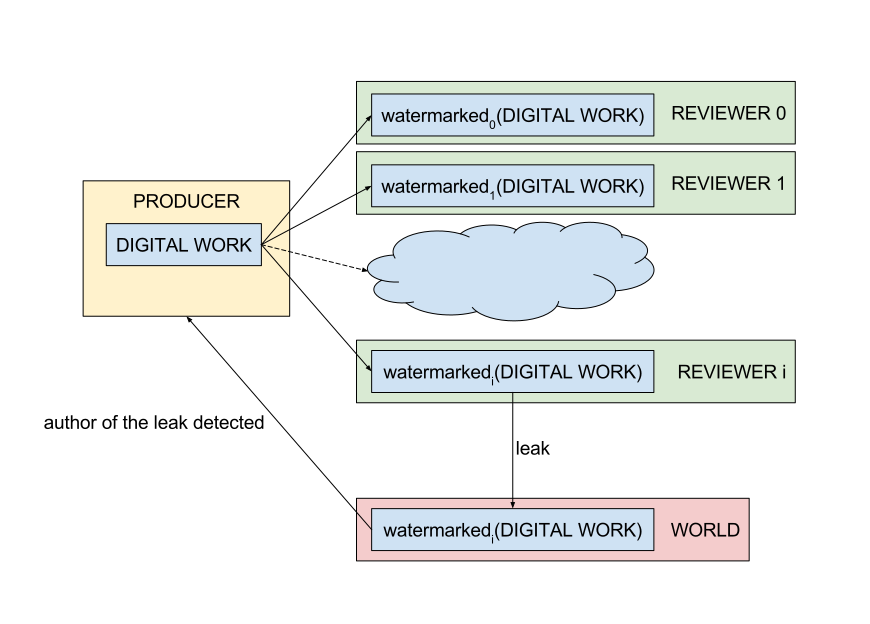
\includegraphics[width=1.0\textwidth]{../../images/simple-leak-detection.png}
  \caption{Schema of a detection process when a work was leaked by a direct user.}
  \label{fig:direct-schema}
\end{figure}

Figure~\ref{fig:direct-schema} explains the solution to presented problem.
Producer who owns a digital work, watermarks every copy of the digital work with
a different watermark and sends the watermarked contents to critics. Whenever
a critic makes a leak, we can identify him by checking if the leaked work
contains a watermarked associated with him. Figure~\ref{fig:direct-leak-ex}
shows a potential image that would be leaked by Paweł Wanat.

\begin{figure}[ht]
  \centering
    \includegraphics[width=1.0\textwidth]{../../images/example-critic.jpg}
  \caption{A picture that would be leaked by Paweł Wanat.}
  \label{fig:direct-leak-ex}
\end{figure}

\subsection*{Content tracking}

Film production company makes movies. They already have a big portfolio that
contains hundreds of digital works. They know that from time to time some
malicious people upload their movies to YouTube. They are very sad about that.
Verifying that a single movie found on YouTube belongs to them is costly,
so before any release they watermark all their movies with single watermark and
they just check, if a movie from YouTube contains their watermark.
\begin{figure}[ht]
  \centering
    \includegraphics[width=1.0\textwidth]{../../images/watermark-tracking.png}
  \caption{Computation work of comparing, when pictures are watermarked and not.}
  \label{fig:tracking-schema}
\end{figure}

On Figure~\ref{fig:tracking-schema}, we can find that the producer has $n$
movies and there are $m$ movies in the Internet that could potentially belong to
the producer. The brute force algorithm would have to compare every producer's
movie with every movie from the Internet. That would give us $n\cdot m$
comparisons. However, if we watermark movies before, then all we have to do
is to check if producer's watermark appears on a movie from the Internet. That
requires merely $m$ checks.

Solution to this problem might be used by photographers who post their photos in
the Internet. It happens frequently that people are reposting their pictures on
their feeds in social media without pointing the source.

\subsection*{End user leak detection}

Film production company made a movie. They want to sell their movie to some end
users, via cinemas or other film brokers. They are afraid that some end user
will find a way to download or record the content and then share it somewhere in
the Internet. They want to secure themselves, so they always can identify
the end user who made a leak. They decided that they will watermark the movie
before sending to any broker and they ask the brokers to watermark it again
before sending to any user. When the leak occur, the company will identify
the broker and the broker will identify the end user.
\begin{figure}[ht]
  \centering
    \includegraphics[width=1.0\textwidth]{../../images/leak-detection-with-a-broker.png}
  \caption{Schema of a detection process when a work was leaked by an end user.}
  \label{fig:end-user-schema}
\end{figure}

Figure~\ref{fig:end-user-schema} explains the process of identifying the user
in case of an Internet streaming film broker. At first we have a first level of
watermarking. We send $wm_i(\text{\footnotesize DIGITAL WORK})$ to broker company $i$ where
$wm_i(\text{\footnotesize DIGITAL WORK})$ denotes watermarked version of {\footnotesize DIGITAL WORK} and
index $i$ ensures that for every broker we watermark the work using different
watermark. Then there is a second level of watermarking when brokers distribute
the work to the end users. When some end user will make a leak then we identify
firstly the broker and the broker identifies the end user.
Figure~\ref{fig:end-user-example} shows a potential image that would be leaked
by Paweł Wanat through Company G.
\begin{figure}[ht]
  \centering
    \includegraphics[width=1.0\textwidth]{../../images/example-end-user.jpg}
  \caption{A picture that would be leaked by Paweł Wanat through Company G.}
  \label{fig:end-user-example}
\end{figure}
  
It is worth to mention how to identify an end user if they recorded hiddenly
the movie in a cinema. At first we would have three layers of watermarking:
company wide watermark, physical address of subordinate, date and room. Then
they would be able to identify the seat of the end user by geometric properties
of recorded screen.
\section{Background}
All the methods shown later will be implemented in source codes for RGB
images. However, for theoretical simplicity, we are considering
grayscale images only, i.e. every pixel is an integer value from 0 to 255.
Another assumption is that all images are of the same size
$width\times height$. Later on, $c$ denotes an image, $c^k$ denotes
$k$-th input image, $c_i$ denotes $i$-th pixel of an image. It is worth to
mention that we are using 2D indices, so when writing $i$-th pixel, the
variable $i$ is 2D. Let $w$ be a vector in
$\{1, -1\}^{width\times height}$ space, called a watermark and let $W$ be
a random vector uniformly distributed over $\{1, -1\}^{width\times height}$. In the source codes we will be treating
a watermark as a $2$-color image, where a black pixel $i$ denotes $w_i = 1$ and a
white pixel $i$ denotes $w_i = -1$. Below we list these definition and
additional ones, so you can return to then quickly, if you forget any.\\
\indent $iff$ -- if and only if\\
\indent $abs(x) = -x$ if $x < 0$ else $x$\\
\indent $w$ -- watermark, $w_i$ in $\{-1, 1\}$\\
\indent $c$/$c^k$ -- content image/$k$-th content image\\
\indent $c_i$/$c^k_i$ -- value of pixel $i$ in image $c$/$c^k$; $c_i$/$c^k_i \in \{0, 1, \ldots, 255\}$\\
\indent $E(X)$ -- expected value of random variable $X$\\
\indent $Var(X)$ -- variance of random variable $X$\\
\indent $W$ -- random watermark\\
\indent $A\cdot B = \sum_i A_i B_i$ -- dot product\\
\indent $lc(A, B) = linear\_correlation(A, B) = \frac{A\cdot B}{length(A)}$\\
\indent Chebyshev's inequality: $Pr(|X-E(X)| >= \epsilon) <= \frac{Var(X)}{\epsilon^2}$\\
By watermarking system we understand a pair of an embedding algorithm and
a detecting algorithm. Figure~\ref{fig:background-schema} describes data flow in
a watermarking system. At first embedding algorithm takes a digital content and
a watermark. Having them, it produces a watermarked version of the digital
content. The detecting algorithm takes a watermark and some digital content.
If the digital content contains the watermark, then it returns "Yes",
otherwise "No". The solid line presents data flow for embedding algorithms. The
dashed and dashed-dotted lines presents data flow for detecting algorithms when
the answer is positive. The dotted and dashed-dotted lines presents data flow
for detecting algorithms when the answer is negative.

\begin{figure}[ht]
  \centering
    \includegraphics[width=1.0\textwidth]{../../images/embedding-detecting-algorithm.png}
  \caption{Embedding and detecting algorithms - work flow.}
  \label{fig:background-schema}
\end{figure}

\section{E\_BLIND/D\_LC watermarking system}

Blind Embedding (E\_BLIND) and Linear Correlation Detection (D\_LC) is the simplest watermarking
system presented in Digital Watermarking and Steganography~\cite{dwas} book.
For this system, a watermark should be randomly generated vector of $\{1, -1\}^{width\times height}$.\\
The \textbf{embedding} algorithm is summation of two matrices. So any pixel in
a watermarked content will differ by $1$ from the original pixel.
\begin{lstlisting}
input: c - an image,
       w - a watemark
output: wc - a watermarked image
algorithm:
  for each pixel i do
    wc[i] = c[i] + w[i]
\end{lstlisting}
The \textbf{detecting} algorithm checks value of linear correlation between
a digital content and a watermark and in case it reaches some threshold
(authors take $0.7$ to get negligibly-small false-positive rate) then it reports
a positive outcome of detection.
In the below code, $N$ denotes number of pixels.
\begin{lstlisting}
input: c - a potentialy watemarked image,
       w - a reference watermark
output: "watermark detected"
          if w appears on c
          else "watermark undetected"
algorithm:
  let lc = sum{c[i]* w[i] : pixel i in watermark} / N
  in
    if lc > 0.7
      then watermark detected
      else watermark undetected
\end{lstlisting}
To get better understanding why it works, we should consider following points:
\begin{enumerate}
\item \label{eblind:reasona} linear correlation between a watermark and itself
      is 1
\item \label{eblind:reasonb} having a watermark randomly generated, linear
      correlation between a watermark and an unwatermarked image is expected to
      be around 0
\item \label{eblind:reasonc} having a watermark randomly generated, linear
      correlation between a watermark and a watermarked image is expected to be
      around 1
\end{enumerate}
Point~\ref{eblind:reasona} is true because
    $lc(w, w) = \frac{\sum_i w_i\cdot w_i}{N} = \frac{\sum_i 1}{N} = 1$.\\
To show point~\ref{eblind:reasonb}, we take random watermark $W$ and we consider
    $abs(E(lc(W, c))) = abs(E(\frac{W\cdot c}{|W|}))$. Observe that $W\cdot c$ is random walk
    around $0$, cause $c_i$ is magnitude $W_i$ is direction, all $W_i$ are
    mutually independent and $Pr(W_i = -1) = Pr(W_i = 1) = 0.5$. Thus
    $abs(E(W\cdot c))$ is likely to be upper bounded by $const\cdot \sqrt{N}$
    and so $abs(E(lc(W, c)))$ is likely to be upper bounded by
    $\frac{const}{\sqrt{N}}$. So the point is true.\\
The last point is now simply true:\\
    $lc(c+W, W) = lc(c, W) + lc(W, W) = lc(c, W)  + 1 \approx 1$

Figure~\ref{fig:e-blind-example} show the blind embedding in use. On the top,
you can find a sample watermark. The left bottom picture is before watermarking.
The right bottom one is after watermarking with E\_BLIND method.
\begin{figure}[ht]
\begin{subfigure}{1.0\textwidth}
  \centering
    \includegraphics[width=0.45\textwidth]{../../watermark.png}
  \caption*{A watermark}
\end{subfigure}
\begin{subfigure}{.5\textwidth}
  \centering
    \includegraphics[width=0.9\textwidth]{../../images/example.jpg}
  \caption*{Not watermarked picture}
\end{subfigure}
\begin{subfigure}{.5\textwidth}
  \centering
    \includegraphics[width=0.9\textwidth]{../../images/example_watermarked.png}
  \caption*{Watermarked picture}
\end{subfigure}
  \caption{Comparison between an unwatermarked work and a watermark one.}
  \label{fig:e-blind-example}
\end{figure}\\
It is impossible to spot a difference with the naked eye between two bottom
images. For the purpose of this document, we are saving
files in a bitmap so the compression not to eat the watermark.

It is worth to mention that E\_BLIND allows to subtract a watermark from
an image, i.e. $wc_i = c_i - w_i$, but then D\_LC compares threshold to
$abs(lc(c, w))$ instead of $lc(c, w)$. This is a mechanism to pass a hidden message to
a watermarked content. Basically, if we watermark with $wc_i = c_i + w_i$
formula then it means message $0$, if we use $wc_i = c_i - w_i$ formula then it means
message $1$. To read the message from the watermarked content, we just check if
linear correlation is positive or negative.
\section{Breaking E\_BLIND}

We define here two probabilistic objects: Random Picture Model and
Natural Picture Model. \textbf{Random Picture Model} is a probability space over the set
of images in which
\begin{itemize}
  \item the value of every pixel has uniform distribution on $\{0, 1, ..., 255\}$
  \item the values are mutually independent
\end{itemize}
\textbf{Natural Picture Model} is a probability space over the set of images
that is induced by reality. So we don't really know how it looks like, but we
will try to observe some of it's properties and then based on the analysis of
Random Picture Model we will try to make some conclusions.\\
Let us present the trick that will break the E\_BLIND method. Basically, in
Random Picture Model if we take random picture $C$ and if we pick two
adjacent pixels $i$ and $j$ from the picture then
\begin{equation}
\label{trick1}
Pr(C_i > C_j) = Pr(C_i < C_j).
\end{equation}
However, if the image $C$ is watermarked with E\_BLIND (so $C = O + w$, for some $O$ from RPM) and if $w_i > w_j$ then
\begin{equation}
\label{trick2}
Pr(C_i > C_j) = Pr(C_i < C_j) + \varepsilon,
\end{equation}
for some $\varepsilon > 0$ that is common for every $i$ and $j$.

Let us take a set of input images -- a set of cardinality $B$. For every two
adjacent pixels $i$ and $j$, we focus on average over all images of
$sgn(C_i-C_j)$. We prove that $E(avg_k(sgn(C^k_i-C^k_j)))$ is equal to
$\varepsilon$ when $w_i > w_j$ and is $0$ when $w_i = w_j$. What is more,  we
show that $Var(avg_k(sgn(C^k_i-C^k_j))) = O\left(\frac{1}{B}\right)$ which is
very small, if we have $B$ big enough. Based on $avg_k(sgn(C^k_i-C^k_j))$, we
would like to predict all the differences of $w_i-w_j$, for all adjacent pixels
$i$ and $j$. That might be hard, so we would be satisfied if we predict $90$\% of
differences correctly. We call our prediction of these differences --
$delta$. Having $delta$ computed, we try to approximate embedded watermark.\\
Until now, we had consideration on random variables. To make it understandable
from a computer perspective, we set $C^k = c^k$ and we compute $delta$. Then we
have heuristic algorithms that can produce a watermark from $delta$.\\
We prove that the prediction of $w_i-w_j$ differences is correct on the level of $90$\%.
Unfortunately we cannot proof any of above for Natural Picture Model. However,
we proceed to treat images the same way and then we make a small
adjustment that solves the problem. Finally, We explore how well the
breaking algorithm is in reality.\\

The algorithm have two steps:
\begin{enumerate}
    \item Computing $delta$.
    \item Computing an approximated watermark form $delta$.
\end{enumerate}
\subsection{Defining $delta$}

We are considering images of certain size $width\times height$. We define
$delta(i,j)$ iff pixel $i$ is adjacent to pixel $j$. We want to claim value
$delta(i, j)$ that will denote our prediction about the watermark difference on
pixel $i$ and $j$, i.e. $w_i + delta(i, j) = w_j$ if we predicted correctly.
\subsection{Computing $delta$}

Let us recall that $B$ is the number of pictures in the input set.
For both Random Picture Model and Natural Picture Model we consider $\{C^k\}_k$.
These are random variables that describe a set of input images. Then
for any adjacent pixels $i$ and $j$ we
define:\\
$X^k_{ij} =
\left\{
\begin{matrix}
1 & \text{, if } C^k_i > C^k_j\\
0 & \text{, if } C^k_i = C^k_j\\
-1 & \text{, if } C^k_i < C^k_j
\end{matrix}\right.\\
Y_{ij} = \frac{\sum^B_k X^k_{ij}}{B}$\\
We will explore values of $E(Y_{ij})$ and $Var(Y_{ij})$ to get some conclusions
about the $delta$.\\
Let us jump to Random Picture Model and let $p_l = Pr(X^k_{ij} = l)$ then:\\
$p_0 = \frac{1}{256}$\\
$p_1 \stackrel{(\ref{trick1})}{=} p_{-1} = \frac{1-p_0}{2} = \frac{255}{512}$\\
$E(X^k_{ij}) = 1\cdot p_1 + 0\cdot p_0 + (-1)\cdot p_{-1} = 0$\\
$E(Y_{ij}) = 0$\\
$Var(Y_{ij}) = \frac{Var(\sum^B_k X^k_{ij})}{B\cdot B} = \frac{Var(X^1_{ij})}{B} = \frac{p_1 + p_{-1}}{B} = \frac{255}{256\cdot B}$\\
Let us see how $Y_{ij}$ behaves when input is a set of watermarked pictures with
the same watermark. We have $C^k = O^k + w$ as input.\\
In case $w_i > w_j$ then\\
$X^k_{ij} =
\left\{
\begin{matrix}
1 & \text{, if } O^k_i + w_i > O^k_j + w_j\\
0 & \text{, if } O^k_i + w_i = O^k_j + w_j\\
-1 & \text{, if } O^k_i + w_i < O^k_j + w_j
\end{matrix}\right.$\\
\begin{align*}
p_1 &= Pr(X^k_{ij} = 1) = Pr(O^k_i + w_i > O^k_j + w_j) =\\
    &= Pr(O^k_i + 2 > O^k_j) =\\
    &= \sum_{l=0}^{255} Pr(O^k_i + 2 > O^k_j | O^k_j = l)Pr(O^k_j = l) =\\
    &= \left(1 + \sum_{i=1}^{255} \frac{257-i}{256}\right)\cdot \frac{1}{256} = \frac{33151}{65536}\approx 0.506\\
p_0 &= Pr(O^k_i + 2 = O^k_j) = \sum_{l=0}^{255} Pr(O^k_i + 2 = O^k_j | O^k_j = l)Pr(O^k_j = l)\\
    &= \sum_{l=2}^{255} Pr(O^k_i + 2 = O^k_j | O^k_j = l)Pr(O^k_j = l)\\
    &= \frac{254}{65536} \approx 0.004\\
p_{-1} &= 1 - p_0 - p_1 = \frac{32131}{65536} \approx 0.49
\end{align*}\\
Thus the expected value and the variance are equal to:
\begin{align*}
E(Y_{ij}) &= E(X^k_{ij}) = p_1 - p_{-1}=\frac{255}{256}\cdot \frac{1}{64}\\
Var(Y_{ij}) &= \frac{Var(X^k_{ij})}{B}\\
            &= \frac{p_1(1-p_1+p_{-1})^2 + p_0(p_1-p_{-1})^2 + p_{-1}(1+p_1-p_{-1})^2}{B}\\
            &= \frac{p_1 + p_{-1} + (p_1-p_{-1})^2}{B}\\
            &\approx \frac{0.996}{B}
\end{align*}
From equation (\ref{trick2}) we know $p_1 - p_{-1} = \varepsilon$ and thus
\begin{equation}
\label{eq:avg:eps}
E(avg_k(sgn(C^k_i-C^k_j))) = E(Y_{ij}) = \varepsilon.
\end{equation}
In case $w_i = w_j$ then it is like there were no watermark, so:\\
\begin{align*}
p_0 &= \frac{1}{256}\\
p_1 = p_{-1} &= \frac{255}{512}\\
E(Y_{ij}) &= 0\\
Var(Y_{ij}) &= \frac{255}{256\cdot B} \approx \frac{0.996}{B}
\end{align*}
In case $w_i < w_j$ then $Y_{ij} = -Y_{ji}$ so:\\
\begin{align*}
E(Y_{ij}) &= -\frac{255}{256}\cdot \frac{1}{64}\\
Var(Y_{ij}) &= \frac{p_1 + p_{-1} + (p_1-p_{-1})^2}{B} \approx \frac{0.996}{B}
\end{align*}
Having the expected values of $Y_{ij}$ computed we obtained a natural predicate
that gives $delta$. Basically, we set:\\
$delta(i, j) = \left\{
  \begin{matrix*}[l]
    2&\text{, if } Y_{ij} < -\tau\\
    0&\text{, if } -\tau <= Y_{ij} <= \tau\\
    -2&\text{, if } \tau < Y_{ij}
  \end{matrix*}\right.$ , where $\tau = \frac{\varepsilon}{2}$\\
Let us apply Chebyshev's inequality to $Pr(|Y_{ij} - E(Y_{ij})| >= \tau)$:
$$
Pr(|Y_{ij} - E(Y_{ij})| \geq \tau)
  \leq \frac{Var(Y_{ij})}{\tau^2}
  \leq \frac{1}{B\tau^2}
  = \frac{256\cdot 256\cdot 128\cdot 128}{255\cdot 255\cdot B},
$$
so if $B > 166000$ then $Pr(|Y_{ij} - E(Y_{ij})| >= \tau) <= 0.1$ and thus
$90$\% of $delta$ is correctly predicted. The number $166000$ is only an upper bound. Experiments shows
that we need much less pictures to get good results (see section~\ref{sec:performance}).\\
The way to deduce $delta$ from the input data is to take $C^k = c^k$ and
evaluate $delta$ based on that.

\subsection{Computing an approximated watermark form $delta$}

In this section two algorithms are described. Both of them are heuristic,
but we will see that they give good results, i.e. the fraction of correctly
predicted pixels of watermark is large enough. The first algorithm is for
CPU and the other one is for GPU. Both of them use $update$
function, which basically should transform a current solution to
a better one. The GPU version execute many updates in parallel, so we need
to take care that all threads are synchronized well.\\
At first, we consider relaxed problem, i.e. having $delta$, we want to determine
a correspondent vector $w'$ in $[-1, 1]^{width\times height}$. Then we start by
setting $w' = 0$. We perform some updates in order defined later.
Having updated vector $w'_i$ computed, we return $w$ as an approximated watermark 
where:
$$w_i = \left\{
\begin{matrix}
1 & \text{, if } w'_i > 0\\
-1 & \text{, otherwise}
\end{matrix}\right.$$
Let us describe the $update$ function. It gets adjacent pixels $i$ and $j$ 
plus a current solution $w'$ as an input and modify provided $w'$ so that:
\begin{itemize}
  \item the value $w'_k$ remains untouched for $k$ different than $i$ and $j$
  \item let $sum = w'_i + w'_j$ and let $delta'$ be the closest number to $delta(i,j)$ such that
    \begin{enumerate}
      \item $abs(delta') \leq abs(delta(i,j))$
      \item $\frac{sum + delta'}{2} \in [-1,1]$
      \item $\frac{sum - delta'}{2} \in [-1,1]$
    \end{enumerate}
    then $w'_i = \frac{sum - delta'}{2}$ and $w'_j = \frac{sum + delta'}{2}$
\end{itemize}
Such $delta'$ always exists because $delta' = 0$ fulfills these conditions.
To formalize the above, we give a pseudocode.
\begin{lstlisting}
  def update(w', i, j):
    sum = w'[i] + w'[j]
    delta' = max(min(delta(i, j), 2 - sum, 2 + sum),
                 -2 - sum,
                 -2 + sum)
    w'[i] = (sum - delta') / 2
    w'[j] = (sum + delta') / 2
\end{lstlisting}
Note that $update$ procedure preserves invariant that sum of $w'_i$ over all
pixels $i$ equals $0$. It is important for GPU solution to perform updates in a such
way that no pixel is updated at the same time by two or more calls.\\
Let us see an example of several updates on initiated $w' = 0$. We start with:\\
$$\begin{bmatrix}
0 & 0 & 0\\
0 & 0 & 0\\
0 & 0 & 0
\end{bmatrix}$$
Let us pick two adjacent pixels to update:
$$\begin{bmatrix}
0 & 0 & 0\\
\textbf{\color{blue} 0} & \textbf{\color{blue} 0} & 0\\
0 & 0 & 0
\end{bmatrix}$$
Assume that $delta = 2$ for these pixels then the updated solution $w'$ is:
$$\begin{bmatrix}
0 & 0 & 0\\
-1 & 1 & 0\\
0 & 0 & 0
\end{bmatrix}$$
Let us pick another two adjacent pixels:
$$\begin{bmatrix}
0 & 0 & 0\\
-1 & \textbf{\color{blue} 1} & 0\\
0 & \textbf{\color{blue} 0} & 0
\end{bmatrix}$$
Assume that $delta = 0$ for these pixels then:
$$\begin{bmatrix}
0 & 0 & 0\\
-1 & 0.5 & 0\\
0 & 0.5 & 0
\end{bmatrix}$$
And so on.\\
\begin{figure}[ht]
  \centering
    \includegraphics[width=1.0\textwidth]{../../images/horizontal-phases.png}
  \caption{Horizontal phases}
  \label{schema:horizontal-phases}
\end{figure}
For CPU we randomly pick adjacent pixels $i$ and $j$ to
perform $update$ on them. 
\begin{lstlisting}
  for every pixel i: set w'[i] = 0
  repeat (10*width*height) times:
    i, j = pick_adjacent_pixels_at_random(width, height)
    update(w', i, j)
  get w from w'
\end{lstlisting}

On GPU we have a different approach. We want to make parallel $update$ calls and
do it in such way that in the same time no two updates would intersect. To make
this happen, we call some of pixels active and the rest call inactive.
Iteratively, we perform horizontal phases and vertical phases. On
Figure~\ref{schema:horizontal-phases} and~\ref{schema:vertical-phases} phases are
shown. Yellow pixels are the active ones. On their behalf, updates are
performed. In a horizontal phase, every active pixel perform an update on
itself and their right neighbour. In a vertical phase, every pixel perform
an update on itself and their bottom neighbour. In first horizontal phase,
the first column consists of active pixels and so every second column. In second
horizontal phase active pixels are these, which were inactive in the first
phase. If a number of columns is odd then pixels from the last column are inactive
in both horizontal phases. For vertical phases, active pixels are grouped
similarly but in rows.
\begin{figure}[ht]
  \centering
    \includegraphics[width=1.0\textwidth]{../../images/vertical-phases.png}
  \caption{Vertical phases}
  \label{schema:vertical-phases}
\end{figure}
In the following code $get\_id\_*$ returns the id of active pixel for a thread.
Methods $me\_and\_[right|bottom]$ take the first pixel and return a pair of pixels:
the one provided and right or bottom one, respectively.
\begin{lstlisting}
  for every pixel i: set w'[i] = 0
  repeat 10 times:
    parallel update(w', me_and_right(get_id_horizontal_1st()))
    parallel update(w', me_and_bottom(get_id_vertical_1st()))
    parallel update(w', me_and_right(get_id_horizontal_2nd()))
    parallel update(w', me_and_bottom(get_id_vertical_2nd()))
  get w from w'
\end{lstlisting}
\subsection{Performed test}

\textit{Input:} A set of $636$ pictures took mostly by GoPro Hero camera and
Samsung Galaxy Nexus phone.\\
\textit{Description:} The same watermark was embedded into all photos. The CPU
version of breaking algorithm computed an approximation of the underlying
watermark.\\
\textit{Result:} \textbf{77,5\%} correctly predicted pixels.\\
Figure~\ref{fig:red-green-pixels} shows how the breaking algorithm managed to
predict pixels of the embedded watermark. The green dots denote pixels predicted
correctly and the red dots denote the ones predicted wrongly.
\begin{figure}[ht]
  \centering
    \includegraphics[width=1.0\textwidth]{../../images/hidden_watermark-diff.png}
  \caption{Correctly predicted pixels - green, wrongly predicted pixels - red}
  \label{fig:red-green-pixels}
\end{figure}\\
It turns out we can do something better. The things, which might have gone wrong are:
\begin{itemize}
  \item Wrongly predicted watermark from $delta$.
  \item Too small set of pictures. 636 instead of 166000.
  \item We applied solution for Random Picture Model to Natural Picture Model
\end{itemize}
Could the watermark be predicted wrongly from $delta$? To verify this another
test was performed in which we run the breaking algorithm on a set of
images that contained exactly one picture, which was a watermark itself.
The solution predicted less that $1$\% of pixels correctly, which is very good
result (In case the algorithm predicts $50$\% of pixels correctly then it
means that if works randomly, $0$\% and $100$\% correctness are expected
mostly). So first dot is not a case.\\
Could the set be too small. Yes, it could. However, it is hard to test the
solution on a larger set. The CPU solution is executing almost an hour for $636$
pictures and current implementation of GPU solution requires more device memory.
More pictures - more resources needed to verify. So the second dot might be the
case, but we won't verify it.
\begin{figure}[ht]
  \centering
    \includegraphics[width=1.0\textwidth]{../../images/histograms/hori.png}
  \caption{Histogram of horizontal $Y_{ij}$ values}
  \label{hist:hori-y}
\end{figure}\\
For the third dot the answer is: yes, it is the case. To understand that imagine
how a histogram for $Y_{ij}$ would look like. It should have $3$ peaks
around $\frac{1}{64}$, $0$ and $-\frac{1}{64}$. The first peak comes from pixels
$i$ and $j$ where $w_i > w_j$
(from equation (\ref{eq:avg:eps}) we have
$E(Y_{ij}) = \varepsilon \approx \frac{1}{64}$), the second is
when $w_i = w_j$ and the last when $w_i < w_j$. Let us take a look on
a histogram of $Y_{ij}$ horizontal values that was generated on a real data --
the set of 636 images. It is presented on Figure~\ref{hist:hori-y}
We see the peaks around $-0.75$, $0$, $0.75$. The peaks are further than in
Random Picture Model. Setting $\tau$ to $0.3$ (used in $delta$ definition) we
are getting result \textbf{99,6\%} correctly predicted pixels of an embedded
watermark while running on the set of 636 photos. I hope that the location of
the peaks could be understood by considering the histogram of $|C^k_i - C^k_j|$
which looks exponentially, while for Random Picture Model, a distribution is
a triangle.\\
Figure~\ref{fig:delta-histogram} presents the histogram of values
$(C^k_i - C^k_j)$ aggregated over all possible pixels $i$ and $j$, and $4$ images'
indices picked randomly as $k$.
\begin{figure}[ht]
  \centering
    \includegraphics[width=1.0\textwidth]{../../images/histograms/diff_hist_no_water_4pics.png}
  \caption{Histogram of $C^k_i - C^k_j$}
  \label{fig:delta-histogram}
\end{figure}\\
Note that if we make similar histogram for watermarked bitmaps
then it looks quite different what is presented on Figure~\ref{fig:delta-histogram-watermarked}.
\begin{figure}[ht!]
  \centering
    \includegraphics[width=1.0\textwidth]{../../images/histograms/diff_hist_water_4pics.png}
  \caption{Histogram of $C^k_i + w_i - C^k_j + w_j$}
  \label{fig:delta-histogram-watermarked}
\end{figure}
Thus the shape analysis of this histogram might give a suspicion that inside
a set of images there is a watermark embedded with E\_BLIND method.
\section{\label{sec:performance}Experimental convergence speed of\\ the breaking algorithm}
The breaking algorithm was run for every combination
of indices $env$, $B$ and $times$ on sets of watermarked images. The possible values for indices are described by:
\begin{enumerate}
  \item Index $env \in \{\text{CPU}, \text{GPU}\}$
  \item Index $B \in \{1, 5, 9, 13, 17, 21\}$
  \item Index $times \in \{1,2,3\}$ in case of $env=\text{CPU}$ or $times \in \{1,2,3,4,5\}$ in case of $env=\text{GPU}$
\end{enumerate}
Index $B$ denotes that we run the breaking algorithm on a set of cardinality $B$.
Index $times$ denotes number of a sample set of cardinality $B$ that is run on
$env$. We ran the breaking algorithm and computed linear correlations, which then
we averaged over all $times$. So for every $env$ and $B$ we got average linear
correlation. The results was displayed on Figure \ref{lc-benchmark} from left
to right, sorted by $B$.

\begin{figure}[ht!]
  \centering
    \includegraphics[width=1.0\textwidth]{../../images/lc-benchmark.png}
  \caption{lc-convergence speed on CPU and GPU.}
  \label{lc-benchmark}
\end{figure}
\section{Running code}

Generating random watermark:
\begin{lstlisting}
python generate_watermark.py -o watermark
\end{lstlisting}
Watermarking pictures with E\_BLIND:
\begin{lstlisting}
python watermark_pictures.py\
  --in=photos\
  --out=watermarked\
  --watermark=watermark.bmp\
  --usecuda=true
\end{lstlisting}
Computing linear correlation of multiple files against a watermark:
\begin{lstlisting}
python compute_linear_correlation.py\
  --in=watermarked\
  --reference=watermark.bmp
\end{lstlisting}
Finding a watermark embedded in multiple digital works:
\begin{lstlisting}
python break_adj.py\
  --watermarked=watermarked/\
  --deduced=deduced.bmp\
  --size=2592x1944\
  --usecuda=true
\end{lstlisting}
Generating histogram for differences between adjacent pixels:
\begin{lstlisting}
python diffenerce_histogram.py\
  --in=photos/\
  --rangeradius=30
\end{lstlisting}


\section{Execution speed comparision between CPU and GPU}

A test was performed to compare execution speed of CPU and GPU solutions. 
We used \textit{Intel(R) Core(TM) i7-4710HQ CPU @ 2.50GHz} for CPU and
\textit{GeForce GTX 980} for GPU.
\begin{figure}[ht!]
  \centering
    \includegraphics[width=1.0\textwidth]{../../images/time-benchmark.png}
  \caption{Comparison of CPU and GPU execution times.}
  \label{time-benchmark}
\end{figure}
There were 100 runs of both versions. The real time of execution is presented on
Figure~\ref{time-benchmark}. Every run had to process $B$ images, where $B$ was
taken from $1$ to $100$. The times on chart are sorted by $B$ and
displayed from left to right. Fluctuations for CPU solutions might come from the
fact that the solution is using multi processing and the processes have to
synchronized between them, which works in nondeterministic time.
\section{Problems}
\begin{enumerate}
    \item File format: If you take a content and watermark them using E\_BLIND
    and then you save them as JPG then it is more likely that your watermark
    won't survive a compression and will not be visible anymore. So when I use
    E\_BLIND, I save the watermarked content in BMP.
    \item Analysis of breaking algorithm assumes that $C'^k = C^k + w$. In fact,
    $C'^k = max(0, min(255, C^k + w))$. It should be verified that
    $Pr(C'^k = max(0, min(255, C^k + w)) != C^k + w)$ in Random Picture Model.
    \item Understand why peaks and antipeaks are in $-0.75$, $-0.3$, $0$, $0.3$, $0.75$
    when considering Natural Picture Model.
    \item The tests for breaking E\_BLIND accuracy were performed only on one
    watermark. They should be performed on many such watermarks and we should
    claim the averaged accuracy.
    \item Verify if $$Pr(C_i > C_j) = Pr(C_i < C_j)$$ is true for Natural Picture
    Model and if not then approximate the error.
    \item Explore and prove the relation between percentage of $delta$ predicted
        correctly and a lower bound on percentage of correctly predicted pixels
        in an underlying watermark.
        
        
\end{enumerate}
\section{Epilogue}
You can make E\_BLIND resistant from the presented attack if you have a set of
watermarks and you always pick a watermark at random before watermarking any
single picture. In case you are watermarking movie, you should pick a watermark
at random for each frame.

\bibliographystyle{plain}
\bibliography{msc}{}


\newpage
\section*{Supplement - sources}
All the codes for this paper can be found on: {\tiny HTTPS://GITHUB.COM/WANATPJ/H\_BLIND}\\
The name of the repository H\_BLIND means hacking blind embedding - E\_BLIND.\\
\renewcommand{\arraystretch}{1.5}
\addvbuffer[12pt 8pt]{\begin{tabular*}{\textwidth}{|l|p{7.55cm}|}\hline
File & Description \\ \hline\hline
break\_adj.py & Breaking E\_BLIND algorithm. Deduces the watermark, given a set
    of images containing the same watermark embedded with E\_BLIND method.\\ \hline
common.py & Utils\\ \hline
compute\_linear\_correlation.py & Computes linear correlation between a watermark
    and some image or a set of image. In case of set, it returns average linear
    correlation.\\ \hline
cudalib.py & Implementations of GPU kernels and processes that run the kernels\\ \hline
difference\_histogram.py & Computes the histogram of $C^k_i-C^k_j$\\ \hline
generate\_watermark.py & Generates a random watermark\\ \hline
watermark\_pictures.py & Watermarks pictures with a certain watermark using E\_BLIND embedder.\\ \hline
\end{tabular*}}\\
Initially $delta$ was called \textit{edge model}, so whenever you see \textit{edge model}
in the codes, please think of $delta$.
\newpage
\subsection*{break\_adj.py}
\lstinputlisting[language=Python]{../../break_adj.py}
\newpage
\subsection*{common.py}
\lstinputlisting[language=Python]{../../common.py}
\newpage
\subsection*{compute\_linear\_correlation.py}
\lstinputlisting[language=Python]{../../compute_linear_correlation.py}
\newpage
\subsection*{cudalib.py}
\lstinputlisting[language=Python]{../../cudalib.py}
\newpage
\subsection*{difference\_histogram.py}
\lstinputlisting[language=Python]{../../diffenerce_histogram.py}
\newpage
\subsection*{generate\_watermark.py}
\lstinputlisting[language=Python]{../../generate_watermark.py}
\newpage
\subsection*{watermark\_pictures.py}
\lstinputlisting[language=Python]{../../watermark_pictures.py}

\end{document}
